\documentclass[12pt]{article}
\usepackage{ctex}
\usepackage{graphicx}
\usepackage{caption}
\usepackage{tabularx}
\usepackage{geometry}

\geometry{a4paper,scale=0.75}


\title{电力电子技术课程设计}
\author{许文晋}
\begin{document}
\tableofcontents
\pagebreak
\counterwithin{figure}{section}
\counterwithin{equation}{section}

\section{选题背景}
\subsection{自动化技术的发展与意义}
自动化技术发展历史悠久,应用领域广泛。自动化是人们根据科学知识和经验相结合,利用机器实现高效率,高质量,自动化的生产劳动的成果。20世纪70年代,电子技术、传感器技术、控制技术的快速发展推动了自动化技术的发展。特别是计算机的普及使自动化技术有一个质的变化,计算机的发展推动了机器人技术的进步,自动化技术在各个行业的应用越来越广泛。自动化技术的应用提高了劳动效率,提升了产品质量,改善了工作环境。

我国作为一个制造大国,其发展必须是循序渐进的,在这发展的过程中自动化技术的发展是必不可少的。为了更大幅度的提升生产效率,满足日益增长的复杂性生产,自动化技术趋于成熟,这一趋势是无法避免的。

\subsection{YL-335B的自动生产线的基本介绍}
YL-335B的自动生产线由五个基本单元组成,分别是供料单元、加工单元、装配单元、 输送单元和分拣单元,如图1-1是YL-335B的自动生产线布局。我们利用PLC、伺服电机、变频器、组态触摸屏和传感设备,通过PLC控制执行机构,实现生产线工艺流程,利用人机界面进行监视控制,本课题使用的是三菱FX系列PLC,对除分拣站外四个站生产线流程进行设计、调试。对于设备之间的通讯,我们使用三菱FX系列PLC的N:N网络实现工作要求。主要的对输送站为主站,其他单元为从站,互相之间进行响应来实现生产线工艺流程。YL-335B外观如图1-1所示。
\begin{figure}[htbp]
    \centering
    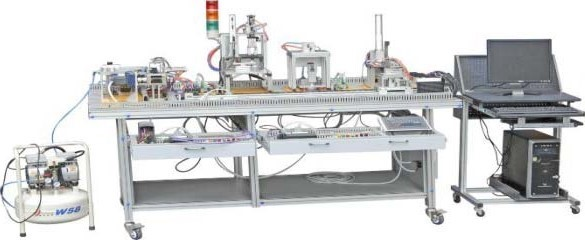
\includegraphics[scale=0.8]{fig/1-1.jpg}
    \caption{YL-335B外观示意图}
\end{figure} 

\section{方案论证(设计理念)}
\subsection{管形料仓}
管形料仓用来存储装配用的金属、黑色和白色小圆柱零件。它由塑料圆管和中空底座构成。塑料圆管顶端放置加强金属环,以防止破损。工件竖直放入料仓的空心圆管内,由于二者之间有一定的间隙,使其能在重力作用下自由下落。 

为了能对料仓供料不足和缺料时报警,在塑料圆管底部和底座处分别安装了2个漫反射光电传感器(E3Z-L型),并在料仓塑料圆柱上纵向铣槽,以使光电传感器的红外光斑能可靠照射到被检测的物料上。如图 2-1 所示。光电传感器的灵敏度调整应以能检测到黑色物料为准则。
\begin{figure}[htbp]
    \centering
    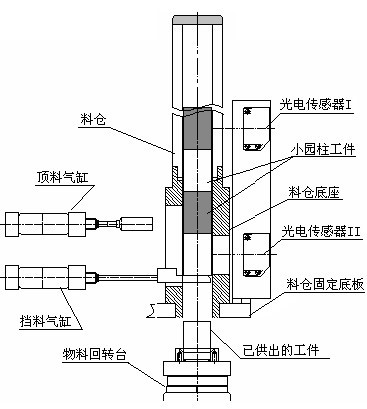
\includegraphics[scale=0.8]{fig/2-1.jpg}
    \caption{落料机构示意图}
\end{figure} 

\subsection{落料机构}
图 2-1 给出了落料机构剖视图。图中,料仓底座的背面安装了两个直线气缸。上面的气缸称为顶料气缸,下面的气缸称为挡料气缸。系统气源接通后,顶料气缸的初始位置在缩回状态,挡料气缸的初始位置在伸出状态。这样,当从料仓上面放下工件时,工件将被挡料气缸活塞杆终端的挡块阻挡而不能落下。需要进行落料操作时,首先使顶料气缸伸出,把次下层的工件夹紧,然后挡料气缸缩回,工件掉入廻转物料台的料盘中。之后挡料气缸复位伸出,顶料气缸缩回,次下层工件跌落到挡料气缸
终端挡块上,为再一次供料作准备。

\subsection{回转物料台}
该机构由气动摆台和两个料盘组成,气动摆台能驱动料盘旋转 180 度,从而实现把从供料机构落下到料盘的工件移动到装配机械手正下方的功能。见图2-2。图中的光电传感器1和光电传感器2分别用来检测左面和右面料盘是否有零件。两个光电传感器均选用CX-441型。
\begin{figure}[htbp]
    \centering
    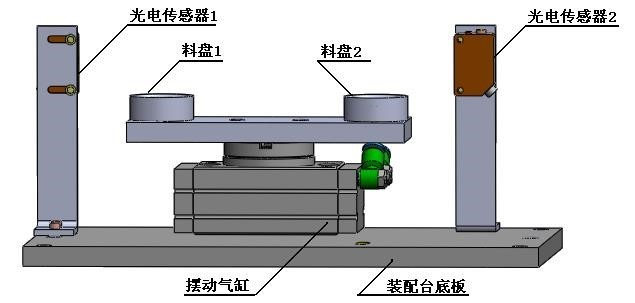
\includegraphics[scale=0.8]{fig/2-2.jpg}
    \caption{回转机构示意图}
\end{figure} 

\subsection{装配机械手}
装配机械手是整个装配单元的核心。当装配机械手正下方的廻转物料台料盘上有小圆柱零件,且装配台侧面的光纤传感器检测到装配台上有待装配工件的情况下,机械手从初始状态开始执行装配操作过程。装配机械手整体外形如图2-3所示。
\begin{figure}[htbp]
    \centering
    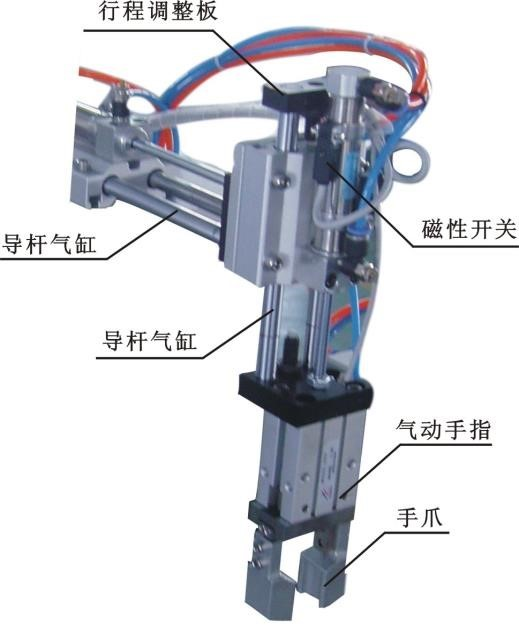
\includegraphics[scale=0.8]{fig/2-3.jpg}
    \caption{装配机械手的整体外形}
\end{figure} 

装配机械手装置是一个三维运动的机构,它由水平方向移动和竖直方向移动的2个导向气缸和气动手指组成。 装配机械手的运行过程如下:

PLC 驱动与竖直移动气缸相连的电磁换向阀动作,由竖直移动带导杆气缸驱动气动手指向下移动,到位后,气动手指驱动手爪夹紧物料,并将夹紧信号通过磁性开关传送给 PLC,在 PLC 控制下,竖直移动气缸复位,被夹紧的物料随气动手指一并提起,离开当廻转物料台的料盘,提升到最高位后,水平移动气缸在与之对应的换向阀的驱动下,活塞杆伸出,移动到气缸前端位置后,竖直移动气缸再次被驱动下移,移动到最下端位置,气动手指松开,经短暂延时,竖直移动气缸和水平移动气缸缩回,机械手恢复初始状态。 

在整个机械手动作过程中,除气动手指松开到位无传感器检测外,其余动作的到位信号检测均采用与气缸配套的磁性开关,将采集到的信号输入 PLC,由 PLC 输出信号驱动电磁阀换向,使由气缸及气动手指组成的机械手按程序自动运行。 

\subsection{装配台料斗}
输送单元运送来的待装配工件直接放置在该机构的料斗定位孔中,由定位孔与工件之间的较小的间隙配合实现定位,从而完成准确的装配动作和定位精度。如图2-4所示。

为了确定装配台料斗内是否放置了待装配工件,使用了光纤传感器进行检测。料斗的侧面开了一个M6的螺孔,光纤传感器的光纤探头就固定在螺孔内。 
\begin{figure}[htbp]
    \centering
    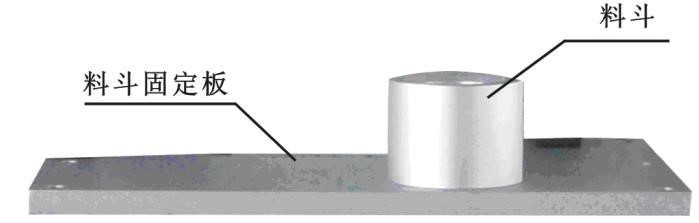
\includegraphics[scale=0.8]{fig/2-4.jpg}
    \caption{装配台料斗}
\end{figure} 

\subsection{警示灯}
本工作单元上安装有红、橙、绿三色警示灯,它是作为整个系统警示用的。警示灯有五根引出线,其中黄绿交叉线为”地线”;红色线:红色灯控制线;黄色线:橙色灯控制线、绿色线:绿色灯控制线;黑色线:信号灯公共控制线。接线如图2-5所示。
\begin{figure}[htbp]
    \centering
    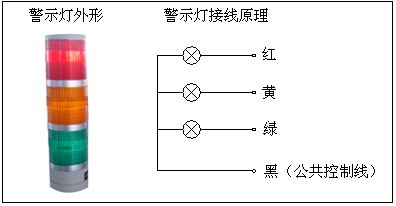
\includegraphics[scale=0.8]{fig/2-5.jpg}
    \caption{警示灯及其接线}
\end{figure} 

\end{document}